\section{反函数与复合函数}
根据\cref{theorem:集合论.关系及其逆是映射的充要条件},
当函数\(f\colon X \to Y\)是单射时,
它有逆映射\(f^{-1}\).
\(f^{-1}\)的定义域和值域分别为\(Z=\ran f\)和\(\dom f=X\).
我们把这个逆映射称为“函数\(f\)的\DefineConcept{反函数}(inverse function)”.
容易证明,\(f^{-1}\)也是定义在\(Z\)上的单调函数.

相对于反函数\(f^{-1}\)来说,
原来的函数\(f\)就称为\DefineConcept{直接函数}.
把直接函数\(y=f(x)\)和它的反函数\(y=f^{-1}(x)\)的图形画在同一坐标平面上,
如\cref{figure:函数.直接函数与反函数的图形的对称性} 所示,
可以看出这两个图形关于直线\(y=x\)是对称的.
这是因为如果\(P(a,b)\)是\(y=f(x)\)图形上的点,
则有\(b=f(a)\).
按反函数的定义,有\(a=f^{-1}(b)\),
故\(Q(b,a)\)是\(y=f^{-1}(x)\)图形上的点;
反之,若\(Q(b,a)\)是\(y=f^{-1}(x)\)图形上的点,
则\(P(a,b)\)是\(y=f(x)\)图形上的点.
而\(P(a,b)\)与\(Q(b,a)\)是关于直线\(y=x\)对称的.

\begin{figure}[ht]
	\centering
	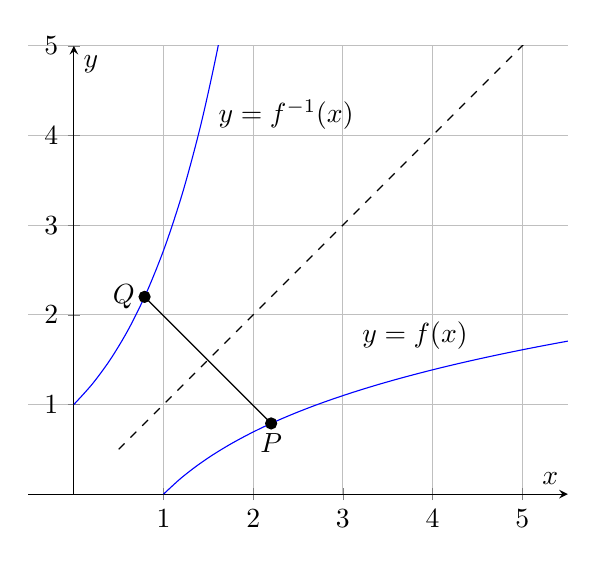
\begin{tikzpicture}
		\begin{axis}[
			xmin=0,xmax=5,
			ymin=0,ymax=5,
			restrict y to domain=0:10,
			grid=both,
			axis equal=true,
			axis lines=middle,
			xlabel=$x$,
			ylabel=$y$,
			axis lines=middle,
		]
			\begin{scope}[color=blue,samples=50,smooth]
				\addplot[domain=0:10]{exp(x)};
				\addplot[domain=1:10]{ln(x)};
			\end{scope}
			\addplot[color=black,dashed,domain=.5:8]{x};
			\filldraw(2.2,{ln(2.2)})circle(2pt)node[below]{$P$}
				--({ln(2.2)},2.2)circle(2pt)node[left]{$Q$};
			\draw(4.5,{ln(4.5)})node[above left]{$y=f(x)$}
				({ln(4.5)},4.5)node[below right]{$y=f^{-1}(x)$};
		\end{axis}
	\end{tikzpicture}
	\caption{}\label{figure:函数.直接函数与反函数的图形的对称性}
\end{figure}

\begin{definition}
设函数\(y=f(u)\)的定义域为\(D_f\),
函数\(u=g(x)\)的定义域为\(D_g\),
且其值域\(R_g \subseteq D_f\),
则函数\[
	y = f[g(x)],
	\quad x \in D_g
\]
称为由函数\(u=g(x)\)与函数\(y=f(u)\)构成的\DefineConcept{复合函数},
它的定义域为\(D_g\),变量\(u\)称为\DefineConcept{中间变量}.

函数\(g\)与函数\(f\)构成的复合函数,
即按“先\(g\)后\(f\)”的次序复合的函数,
通常记为\(f \circ g\),即\[
	(f \circ g)(x) = f[g(x)].
\]
\end{definition}

\begin{example}
设函数\(f\colon(-l,l)\to\mathbb{R}\).
试证:在\((-l,l)\)上必存在偶函数\(g\)和奇函数\(h\),使得\[
	(\forall x)
	[-l<x<l \implies f(x) = g(x)+h(x)].
\]
\begin{proof}
首先假设这样的\(g(x)\)、\(h(x)\)存在,即\[
	f(x) = g(x) + h(x);
	\eqno(1)
\]
于是有\[
	f(-x) = g(-x) + h(-x) = g(x) - h(x).
	\eqno(2)
\]

联立(1)(2)两式,把他们看成是关于\(g(x),h(x)\)的方程,
就可以解得\[
	g(x) = \frac{1}{2} [f(x) + f(-x)], \qquad
	h(x) = \frac{1}{2} [f(x) - f(-x)].
	\qedhere
\]
\end{proof}
\end{example}
